\section{Basic Wireless Network Topologies}
There are 5 types of basic wireless network topologies. These are:

\begin{itemize}
\item{Point To Point}
\item{Star}
\item{Mesh}
\item{Hybrid}
\item{Daisy Chain}
\end{itemize}

\subsection{Point To Point}
A point to point network consists of simply two nodes that are connected to each
other.

\subsection{Star}
A star network (also known as a Point to Multipoint) network has a centralised
controller with nodes connected via point to point connections. In an optical
wireless network this would require the controller to have multiple transmitters
and receivers.

\subsection{Mesh}
A mesh network is where nodes are connected to some (a partial mesh) or all
(a full mesh) of the other nodes in the network.

\subsection{Hybrid}
A hybrid network combines two or more topologies.

\subsection{Daisy Chain}
A daisy chain network connects nodes in series with each other. If they are
connected all together this is known as a 'ring' network.

\subsection{Modelling - Wired versus Wireless}
In wired networks there is also a 'bus' network. However, because wireless
optical communications will be blocked by the receiver, this cannot be factored
in.

If the beam is narrow the network can be thought to act as a 'wired' network
(in that, all connections are point to point only).

If, however, the beam is wider then multiple nodes may be contactable, in which
case we can model this more akin to a wireless access point.

\begin{figure}[H]
  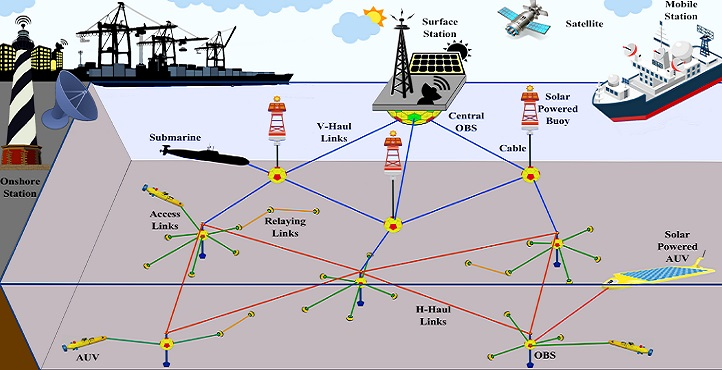
\includegraphics[width=0.8\textwidth]{underwater_network_topologies_v2.jpg}
  \caption{llustration of a generic underwater optical wireless network (UOWN) architecture.}
  \label{fig:underwater_network_topologies_v2}
\end{figure}

\subsection{Underwater versus Terrestrial}
In \cite{s16030414} it is discussed that underwater topologies are highly
dynamic, due to water currents, thus the topology changes frequenctly
(compared to terrestrial networks).

Also, almost all underwater nodes would have to be powered by batteries,
so energy efficient topologies and routing protocols are necessary.

\subsubsection{Always-connected nodes}
In \cite{POMPILI2009778} it is claimed that nodes should coordinate their
depth in such as way to guarantee that the network topology is always connected.
This means there is always a path from every node to the the surface station.

\subsubsection{Tier-based modelling}
In \cite{tier_based_underwater_routing} the topology is partitioned into tiers.
Each node can only select nodes belonging to an upper tier, reducing the
complexity of routing protocols.